
\begin{frame}
\begin{figure}

\vspace{-.7cm}	
\hspace{-2cm}		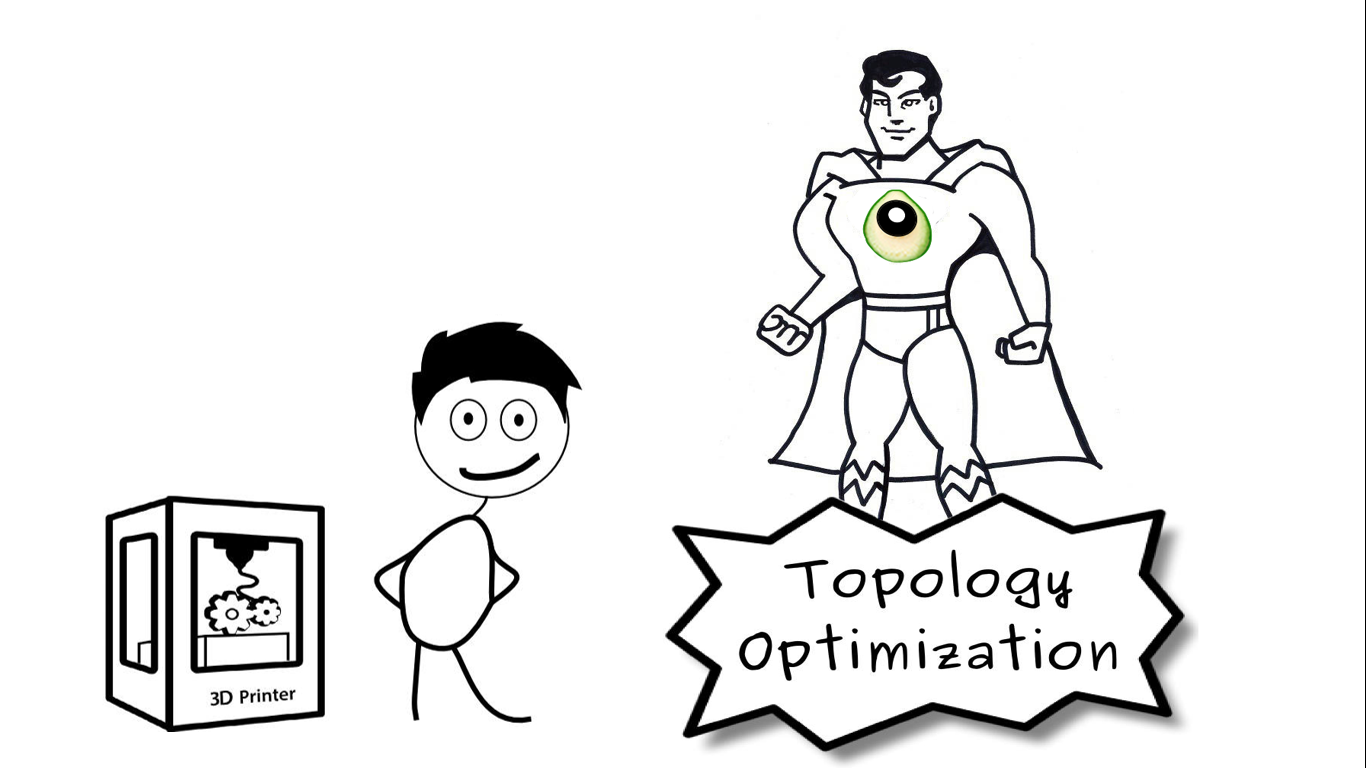
\includegraphics[width=1.2\linewidth]{Pictures/animations/animation_10.png}
		\end{figure}

\end{frame}

\begin{frame}{What is done? What is next?}
%\begin{variableblock}{What's done?}{bg=cyan,fg=white}{bg=white,fg=black}
%{
\begin{itemize}

\item<+-> Topology Optimization
\begin{itemize}
	\item[\textcolor{green}{\Checkmark}] Pipeline from CAD model to optimized voxel model
	\item[\textcolor{green}{\Checkmark}] User input of boundary conditions
	\item[\textcolor{black}{\VarClock}] Support for complex geometries
	\item[\textcolor{red}{\XSolidBrush}] GUI for user interaction
\end{itemize}

\item<+-> Surface Extraction
\begin{itemize}
	\item[\textcolor{green}{\Checkmark}] Dual Contouring for simple geometries
	\item[\textcolor{green}{\Checkmark}] Provide necessary data for Surface Fitting
	\item[\textcolor{black}{\VarClock}] Interfaces
	\item[\textcolor{red}{\XSolidBrush}] Adaptive and topology safe Dual Contouring
\end{itemize}

\item<+-> Surface Fitting
\begin{itemize}
	\item[\textcolor{green}{\Checkmark}] B--spline fitting using least squares
	\item[\textcolor{green}{\Checkmark}] Smooth connection of patches using Peters' scheme
	\item[\textcolor{red}{\XSolidBrush}] Conversion back to CAD
\end{itemize}
\end{itemize}
%}
%\end{variableblock}
\end{frame}
\begin{frame}

	\frametitle{Remaining questions}
	\begin{columns}[c] % The "c" option specifies centered vertical alignment while the "t" option is used for top vertical alignment

	\column{.45\textwidth} % Left column and width
	\begin{block}{Python}
	\begin{itemize}
		\item[{\color{red}$\ominus$}] First part of the pipeline is in C++
		\item[{\color{green}$\oplus$}] Second part of the pipeline is now in Python
		\item[{\color{green}$\oplus$}] Easy to port from the original MATLAB prototypes

	\end{itemize}
	\end{block}

	\column{.45\textwidth} % Right column and width
	\begin{block}{C++}	
	\begin{itemize}
		\item[{\color{green}$\oplus$}] First part of the pipeline is in C++
		\item[{\color{red}$\ominus$}] Second part of the pipeline is now in Python
		\item[{\color{red}$\ominus$}] Cumbersome to implement
	\end{itemize}
	\vspace{3.5mm}

	\end{block}
	\end{columns}
	\pause
	\begin{block}{ToPy Problem}
	\begin{itemize}
	\item[{\color{green}$\oplus$}]<+-> Current implementation is using ToPy
	\item[{\color{red}$\ominus$}]<+-> ToPy is not available any more!
	\end{itemize}
	\end{block}
	
\end{frame}









